The Brushless DC permanent magnet motor design problem was first 
analyzed in \cite{chidambaram1999} as an illustration of a new
catalog-based customization procedure. The same problem formulation 
was analyzed further in \cite{deb2008} to discover innovative 
design principles from the optimization results. We borrow the same 
problem formulation as in \cite{deb2008} for our study.

\section{Problem description}
\label{problem}

A BDCPM motor comprises of an outer stator assembly with windings on a
frame  and inner rotor assembly having pemanently mounted magnets, 
shown in Figures \ref{bdcpmStator} and \ref{bdcpmRotor}. Several 
variants of this basic design exist. The original study 
\cite{chidambaram1999} considered 24 slots 4 pole machine which is 
described next.

\subsection{Motor Schematics}

\subsubsection{Stator Assembly}

The laminations used in this family of BDCPM motors have a thickness 
$t = 5.8 \times 10^{-4} \text{m}$ so that the frame length 
$L = 5.8 \times 10^{-4} n_{l} \text{m}$ where $n_l$ is the number of
laminations. The laminations and the motor frame have $N_s = 24$
slots.

Three lamination types, namely `X', `Y' and `Z' are used in the frame
construction. The variable $L_{type}$ represents the type of 
lamination used in a design. Table \ref{ltypeDimTable} gives the motor
dimensions for different lamination types.

\begin{figure}[ht]\begin{center}
 \fbox{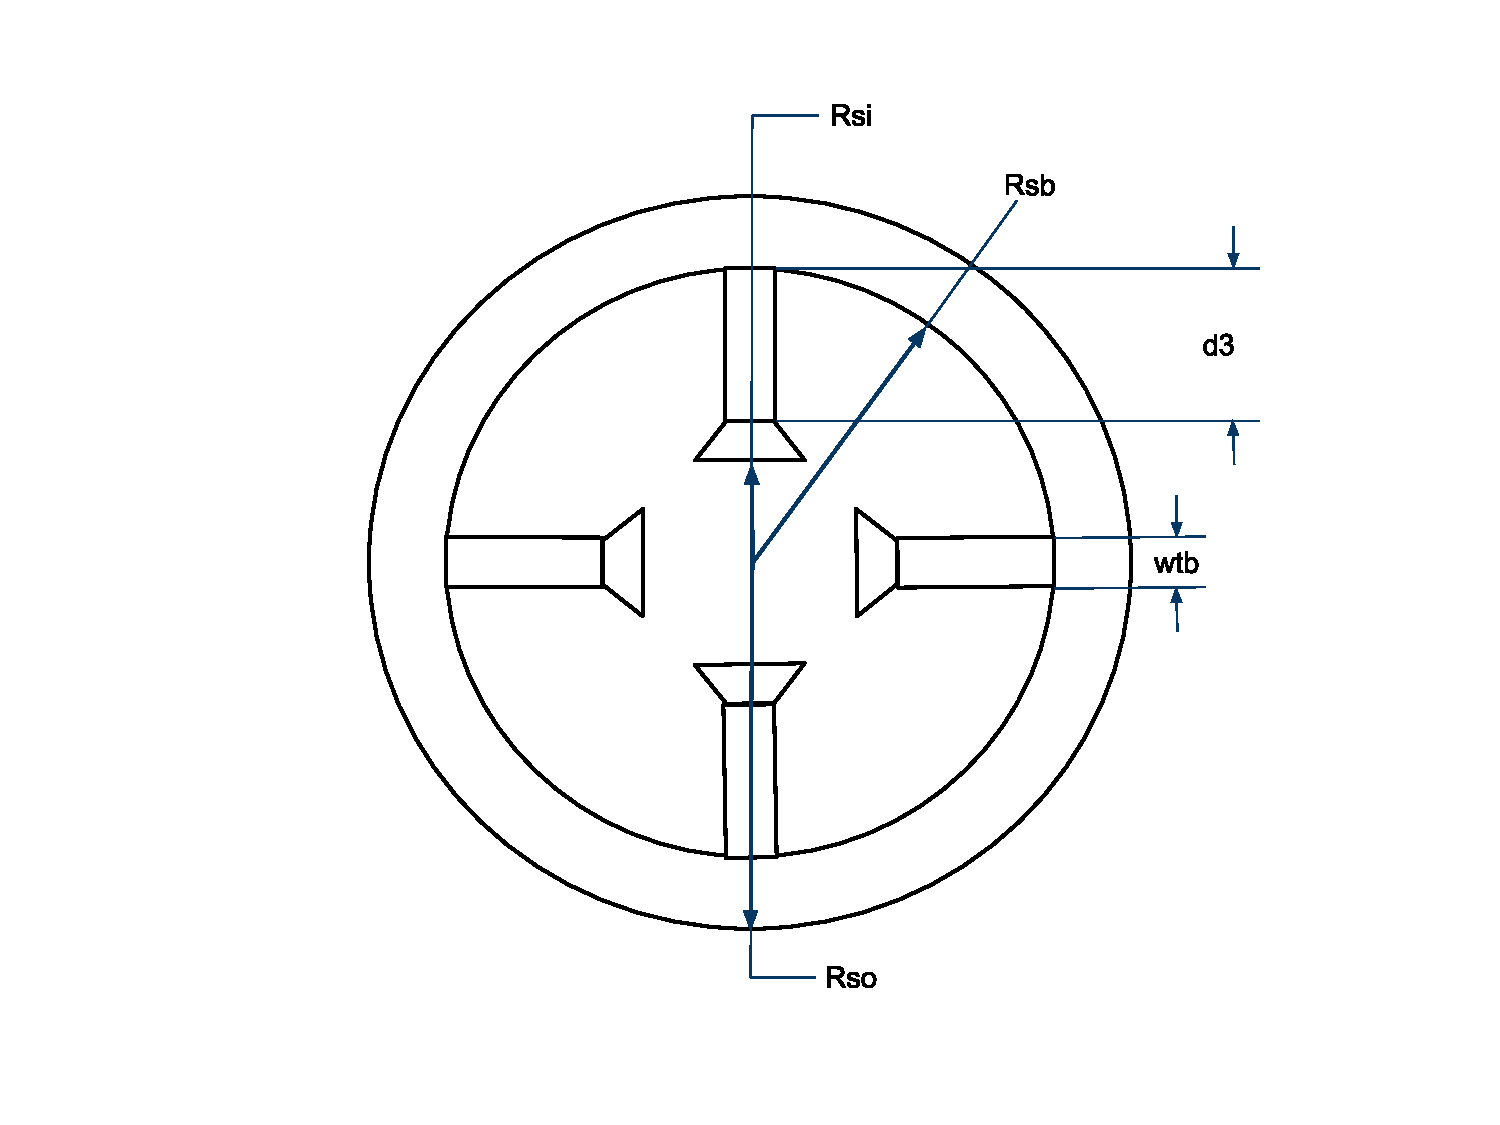
\includegraphics[width=100mm, height=75mm]{diagrams/bdcpmStator.eps}}
 \caption{BDCPMM Stator assembly}
 \label{bdcpmStator}
\end{center}\end{figure}

\begin{table}[!ht]
\centering
\begin{tabular}{|c|c|c|c|c|c|c|c|}
 \hline
 $L_{type}$ & $R_{si}$ (mm.) & $d_3$ (mm.) & $w_{tb}$ (mm.) & $w_{bi}$ (mm.) & $L_{cl}$ (mm.)& $R_{sh}$ (mm.) & $R_{st}$ (m) \\
 \hline
 X & 21.90 & 12.0 & 2.39 & 5.23 & 4.215 & 4.11 & 0.016 \\
 \hline
 Y & 22.22 & 15.1 & 2.39 & 5.23 & 4.265 & 4.11 & 0.016 \\
 \hline
 Z & 25.40 & 15.1 & 2.80 & 5.50 & 4.775 & 4.45 & 0.019 \\
 \hline
 \end{tabular}
\caption{Dimensions of the BDCPM motor family}
\label{ltypeDimTable}
\end{table}




\subsubsection{Rotor assembly}

Figure \ref{bdcpmRotor} shows the rotor assembly of a BDCPM motor. A
ring-magnet is bonded onto a stepped shaft that fits in the bore of
the stator assembly. The total length of the motor is $L_{sh}$. It is 
to be observed that $ L_{sh} = L + 2L_{cl}$. The side clearance 
values, $L_{cl}$ are listed in Table \ref{ltypeDimTable}.


\begin{figure}[ht]\begin{center}
 \fbox{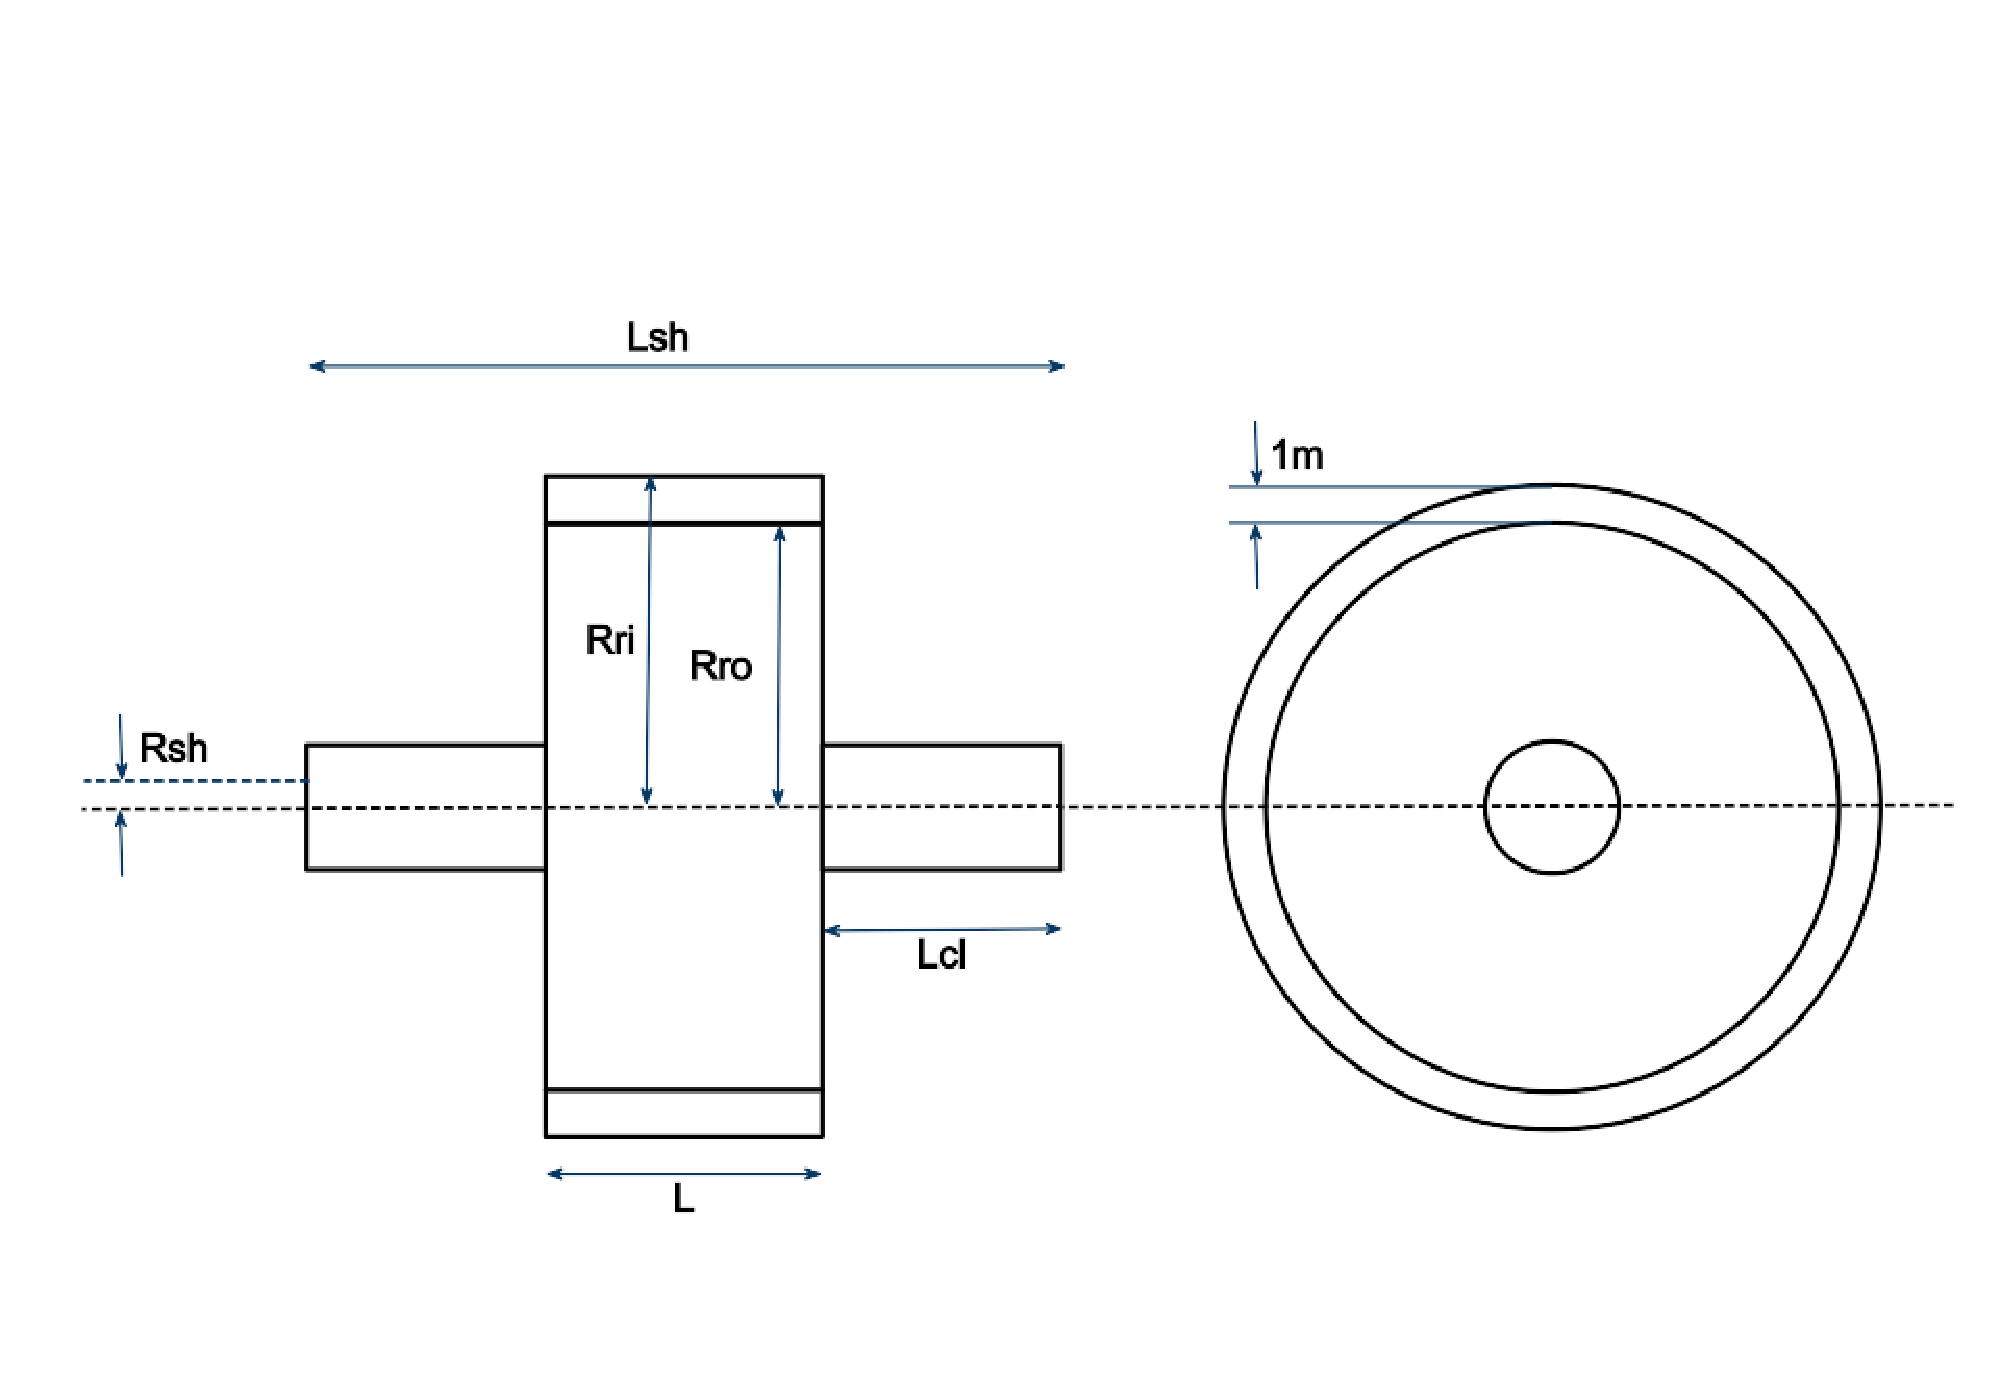
\includegraphics[width=110mm, height=75mm]{diagrams/bdcpmRotor.eps}}
 \caption{BDCPMM Rotor Assembly}
 \label{bdcpmRotor}
\end{center}\end{figure}

\subsection{The Multi-Objecive Optimization Problem}
Two conflicting objecives are considered for BDCPM motor design:

\begin{enumerate}
\item Minimization of manufacturing cost (in \$) of the motor, and
\item Maximization of peak torque (N-m).
\end{enumerate}

Five design variables are considered for the design process, other 
design parameters are fixed to values that are convenient for the 
manufacturer. The design variables are:

\begin{enumerate}
\item Number of laminations $n_l \in [44, 45,\dots ,132]$

\item Number of turns in each coil  $N \in [20, 21, \dots, 80]$

\item $L_{type} \in [\textsf{X, Y, Z}]$ is one of the three types of 
laminations allowed to build the motor

\item $M_{ph} \in [Y, \Delta ]$ is one of the two types of elctric 
connections and

\item $A_{gauge} \in [16, 16.5, 17, \dots , 23.5]$ is one of the 16 
wire gauges used in the windings.
\end{enumerate}

All the design variables are discrete in nature, of which $L_{type}$ 
and $M_{ph}$ take 3 and 2 values respectively. $n_l$ and $N$ are 
integer valued variables while $A_{gauge}$ takes 16 equally spaced 
values in its domain.

The cost expression for the first objecive includes the material and
estimated production cost. Each term in the expression is obtained 
from the regression analyses of data obtained from practice. The 
detailed procedure discribing the derivation of the cost terms and 
torque expressions can be found in \cite{chidambaram1999}.

The actual multi-objective optimization problem is formulated as 
follows:

%%%%%Cost function begins here%%%%%


\begin{singlespacing}

\begin{flushleft}



Minimize   \\
$ C_{total} (n_{l}, N, L_{type}, M_{ph}, A_{wire}) = 
\begin{cases}
\quad 2.6(\frac{n_{l}}{44})^{0.25}, & \text{for $L_{type} =$ X} \\
\quad 0.38 + 2.42(\frac{n_{l}}{44})^{0.37}, & \text{for $L_{type} =$ Y} \\
\quad 1.07 + 1.83(\frac{n_{l}}{44})^{0.58}, & \text{for $L_{type} =$ Z} 
\end{cases} $ \\

$
+  [ \left\{0.026, 0.028, 0.03\right\}n_{l} \cong L_{type} = \{ \textbf{X}, \textbf{Y}, \textbf{Z} \} $\\
$
\, + \, \dfrac{n_{l}}{44} \, + \,   9.8 \times 10^{5} A_{wire} N [ 5.8  \times  10^{-4} n_{l}
   +  \dfrac{\pi}{2} \{ w_{tb} + \dfrac{5\pi}{12}(R_{si} + \dfrac{d_{3}}{2}) \}]
$ \\

$
+ \, 0.3035 \, + \, 0.876 N [ 5.8 \times 10^{-4} n_{l} \, + 
 \dfrac{\pi}{2} \{ w_{tb} \, + \, \dfrac{5 \pi}{12}(R_{si} \, + \, \dfrac{d_{3}}{2})\}]
$\\

$
\, + \, \pi \left[ \left\{ 31.2( R_{si} + d_{3} + w_{bi}) + 0.0312 \right\} \left\{ L_{sh} - 5.08 \times 10^{-3} \right\} \right]
$\\
$
\, + \, 
\begin{cases}
\quad 0.7(\frac{5.8 \times 10^{-4} n_{l} + 0.0792}{0.1047})^{1.21},  & \text{for $L_{type} = $ X} \\
\quad 0.54 + 0.26( \frac{5.8 \times 10^{-4} n_{l} + 0.0802}{0.1057})^{3.74}, & \text{ for $L_{type} =$ Y} \\
\quad 0.58 + 0.32( \frac{5.8 \times 10^{-4} n_{l} + 0.0905}{0.1160})^{4.23}, & \text{ for $L_{type} =$ Z} \\
\end{cases}
$\\
$ \, + \, 9 \, + \, \begin{cases}
\quad 1.3(\frac{5.8 \times 10^{-4} n_{l} + 0.0792}{0.1047})^{0.38} (\frac{n_{l}}{44})^{0.18}, & \text{for $L_{type} =$ X} \\
\quad 1.6(\frac{5.8 \times 10^{-4} n_{l} + 0.0802}{0.1057})^{0.38} (\frac{n_{l}}{44})^{0.40}, & \text{for $L_{type} =$ Y} \\
\quad 1.8(\frac{5.8 \times 10^{-4} n_{l} + 0.0905}{0.1160})^{0.41} (\frac{n_{l}}{44})^{0.52}, & \text{for $L_{type} =$ Z}
\end{cases}
$\\
$
\, + \, (1.536 R_{st} - 6.26 \times 10^{-3}) n_{l} \, + \, (2.014 R_{si} \, - \, 8.21 \times 10^{-3}) n_{l}
$\\
$
\, + \, \pi \{29.4(R_{si} - 7.25 \times 10^{-3})^{2} n_{l} \, + \, 1.014 \times 10^{5} R_{sh}^{2} L_{cl}\} 
$\\
$
\, + \, 0.1862 \, + \, 5.31 \times 10^{4} \pi [ R_{st}^{2} L_{st} \, - \,  2 R_{sh}^{2} L_{cl} 
\, - \, 5.8 \times 10^{-4} n_{l}(R_{si} - 7.25 \times 10^{-3})^{2}] 
$\\
$
 \, + \, 0.01 \, + \,0.1473 \pi (R_{si} - 7.25 \times 10^{-3}) n_{l} \, + \, \begin{cases}
\quad 1.2, & \text{for $T_{p} \le 3.5$} \\
\quad 1.6, & \text{for $T_{p} > 3.5$} 
\end{cases}
$\\
$
\, + \, \left[ \left\{ 0.5, 0.55, 0.60 \right\} \cong L_{type} = \{ \textbf{X}, \textbf{Y}, \textbf{Z} \} \right]
$\\
$
\, + \, \begin{cases}
\quad 3.2(\frac{5.8 \times 10^{-4} n_{l} + 0.0792}{0.1047})^{-1.92}(\frac{n_{l}}{44})^{0.92}, & \text{for $L_{type} = $ X} \\ 
\quad 3.4(\frac{5.8 \times 10^{-4} n_{l} + 0.0802}{0.1057})^{-1.92}(\frac{n_{l}}{44})^{1.06}, & \text{for $L_{type} = $ Y} \\ 
\quad 3.7(\frac{5.8 \times 10^{-4} n_{l} + 0.0905}{0.1160})^{-3.25}(\frac{n_{l}}{44})^{1.60}, & \text{for $L_{type} = $ Z} 
\end{cases}
$
\\[\baselineskip]

%%%%Torque function%%%%

Maximize \\
$ T_p = 87300 C_{tor} N R_{si} A_{wire} n_{l} $\\
where \\
$ C_{tor} = \{ \frac{2}{3}, \frac{1}{3} \} \cong M_{ph} = \{ \textbf{Y}, \Delta  \} $ 
\\[\baselineskip]


Subject to \\
$g_1: T_{p} \geqslant 0.83$ \\

$g_2: T_{p} \leqslant 5.27$ \\

$g_3: A_{wire}N \leqslant \{150, 240, 280\} \times 10^{-7} \cong L_{type} = \{ \textbf{X}, \textbf{Y}, \textbf{Z} \}$

\end{flushleft}

\end{singlespacing}

Constraints $g_1$ and $g_2$ bound the peak torque in the desired 
range. Constraint $g_3$ represents the winding constraints that 
prevent magnetic saturation and demagnetization. Since all the design 
variables are discrete and the objectives vary with the type of 
lamination used, evolutionary approaches to solution are more suitable
for this problem.

\section{Results}

\subsection{Optimization Results}

Since all the variables are discrete, we use binary representation
for them in NSGA-II. We modify the population initialization routine
and the EA operators (recombination and mutation) to maintain the 
discrete nature of the variables. For the two integer valued 
variables, $n_l$ and $N$, discrete version of the Simulated Binary 
Crossover (SBX) and Polynomial Mutation \cite{deb2001} are used. Since
$M_{ph}$ and $L_{type}$ take two and three values only, they are only
subjected to mutation.

Using this representation NSGA-II yeilds 199 non-dominated solutions.
Local search is applied to this set of near optimal solutions to 
achieve better convergence to the true pareto-front. For each 
solution in the NSGA-II output, we evaluate 30 neighboring solution.
After local search, we have a set of 201 non-dominated solutions.
The objective space view of the pareto-front is shown in figure 
\ref{simpParetoB}.
 
 
\begin{figure}[ht]\begin{center}
 \includegraphics[width=100mm, height=80mm]{diagrams/simpParetoB.eps} 
 \caption{Pareto-front for the BDCPMM design problem}
 \label{simpParetoB}
\end{center}\end{figure}


\subsection{Estimating dimensions of the Pareto-front}

\subsubsection{Isomap Residual Variance for the Pareto-front}
On performing Isomap on the pareto-front data of BDCPMM design we 
obtain a residual variance plot shown in figure \ref{isoRVbdcpmAll}. 
Since the residual variance shows a sharp decline going from one 
dimensional embedding to two-dimensional embedding, we can expect the 
pareto-front to be composed of sub-manifolds of one or two dimensions.
There is an unexpected increase in the residual variance for three 
dimensional embedding, though it drops down to the previous level for 
four dimensional embedding. 

\begin{figure}[ht]\begin{center}
 \subfloat[Isomap Residual Variance for the Pareto-front]{
 \label{isoRVbdcpmAll} 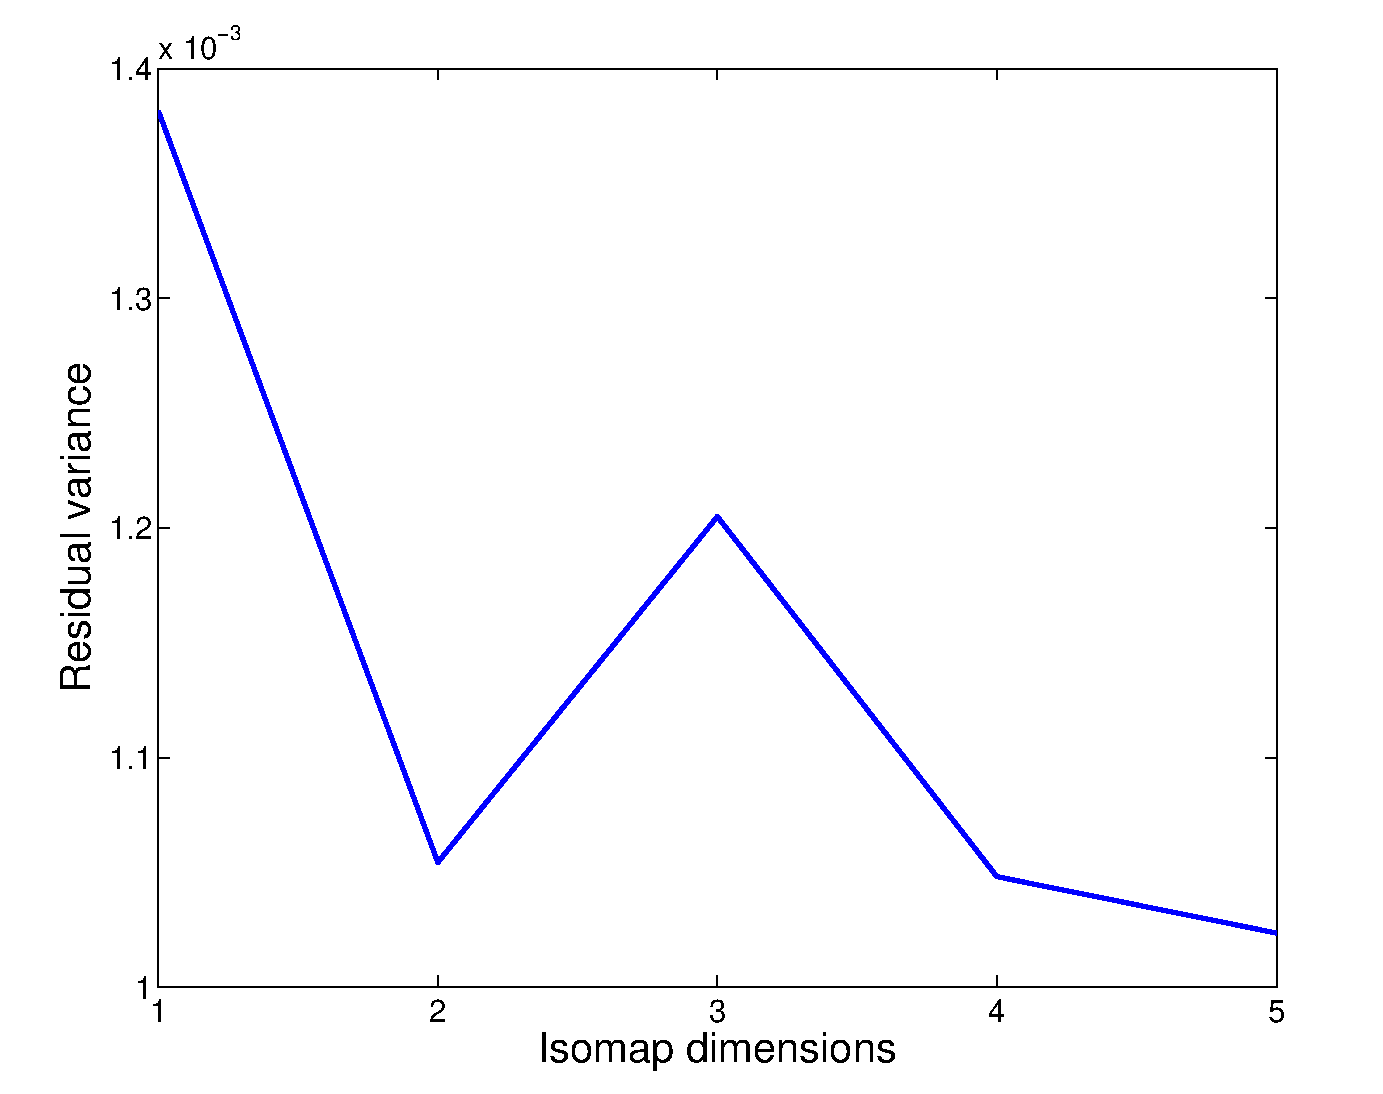
\includegraphics[width=62mm, height=52mm]{diagrams/isoRVbdcpmAll.eps}}
 \subfloat[Explained variance for Principal Components of the Pareto-front]{
 \label{pcaEVbdcpmAll} 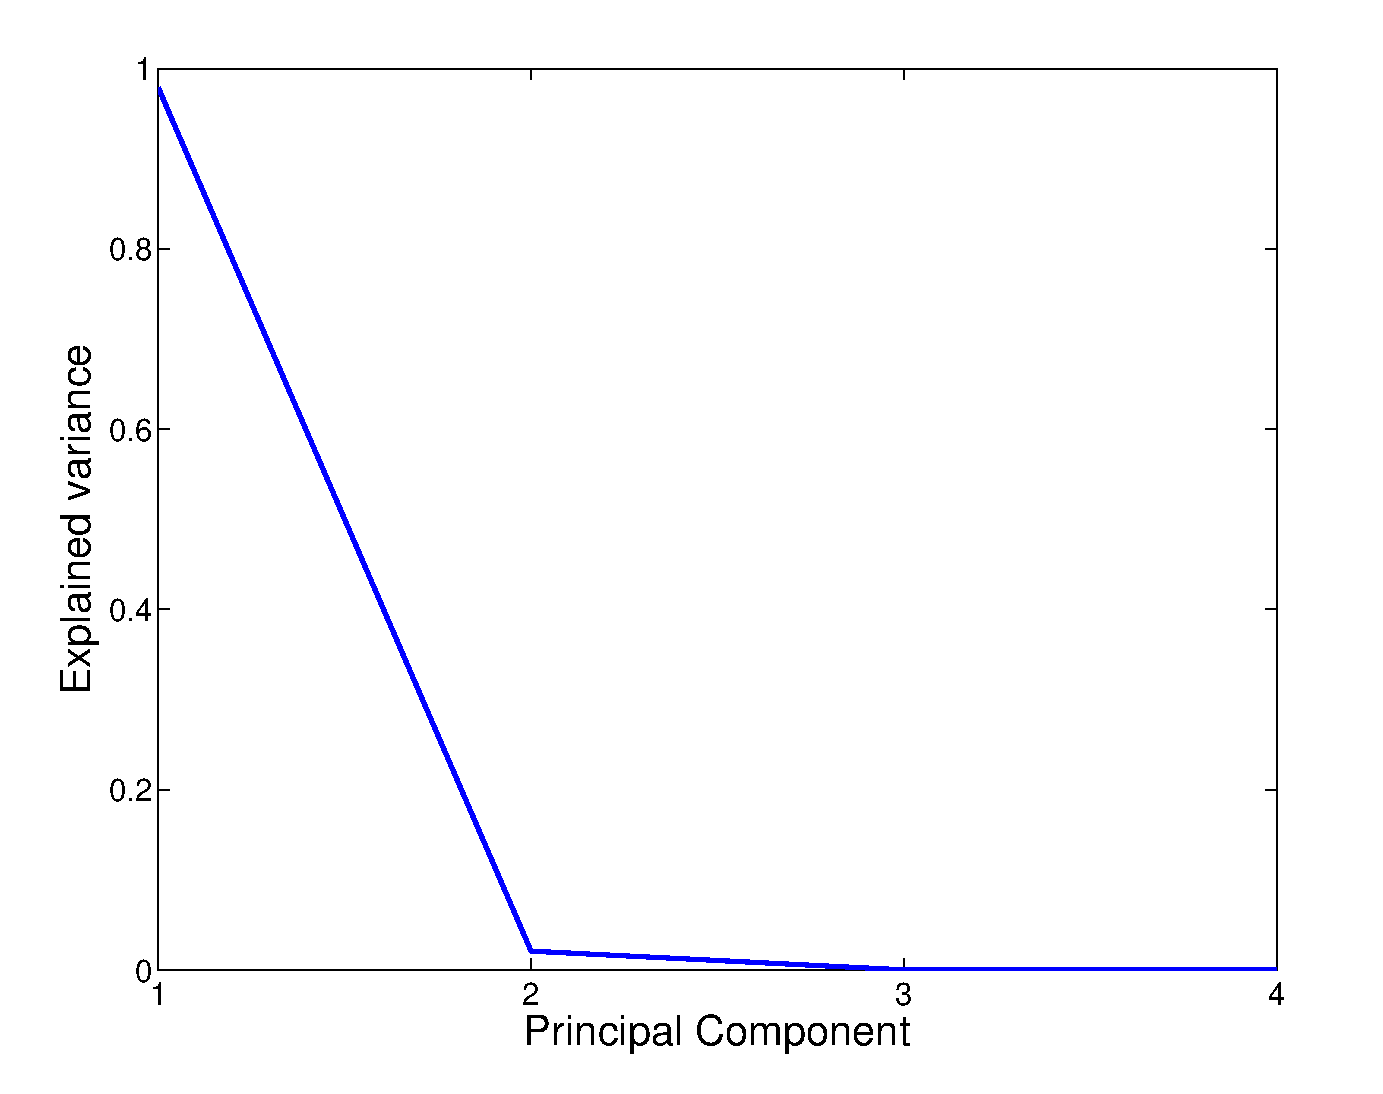
\includegraphics[width=62mm, height=52mm]{diagrams/pcaEVbdcpmAll.eps}}
 \caption{Isomap and PCA results}
 \label{bdcpmmVar}
\end{center}\end{figure}
%%residual variance figure here

\subsubsection{PCA Explained Variance}
The PCA analysis of BDCPMM pareto-front gives four principal 
components.  The explained variance for 
principal components of the BDCPMM pareto-front data are plotted in 
figure \ref{pcaEVbdcpmAll}. The first principal component has 
explained variance of more than 0.95, while the second principal 
component has explained variance of 0.021. The third and fourth 
principal components have negligible explained variances. Table 
\ref{firstTwoPCs} shows the three principal component vectors which 
reveal that the pareto front is a manifold embedded in the plane of 
first two design dimensions, namely number of laminations and number 
of turns in the stator windings.
 

\begin{table}[!ht]
\centering
\begin{tabular}{|c|c|c|c|c|c|}
 \hline
 First PC & 0.9993 & 0.0370 & 0.0072 & 0 & -0.0024\\
 \hline
 Second PC & -0.0367 & 0.9943 & 0.0165 & 0 & 0.0985\\
 \hline
 \end{tabular}
\caption{First two principal components of the BDCPM data}
\label{firstTwoPCs}
\end{table}

\subsection{Clusters in the Pareto-front}
The clustering of the BDCPMM pareto-front results in five clusters 
which are shown in the objecive space plot in figure \ref{bClustersO}. 
Figure \ref{bClustersP} shows the clusters with respect to the number
of laminations and the Wire Gauge used in the stator windings. Other  
design variables are indicated alongside the clusters.


\begin{figure}[ht]\begin{center}
 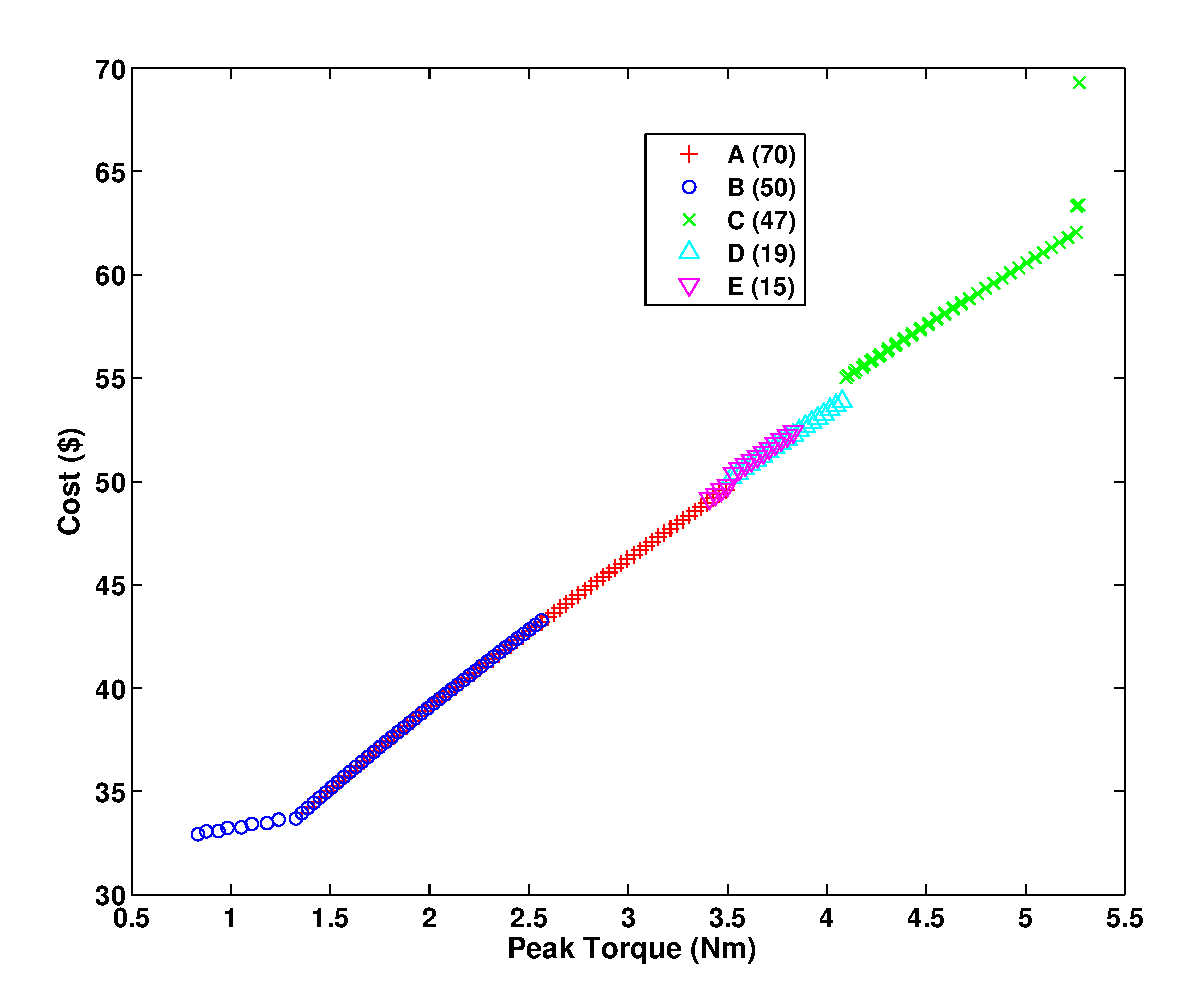
\includegraphics[width=100mm, height=80mm]{diagrams/bClustersO3.eps} 
 \caption{Clusters in the BDCPMM pareto-front}
 \label{bClustersO}
\end{center}\end{figure}


\begin{figure}[ht]\begin{center}
 \includegraphics[width=100mm, height=80mm]{diagrams/bClustersP2.eps} 
 \caption{Clusters in the \#Laminations-Wire-gauge subspace.}
 \label{bClustersP}
\end{center}\end{figure}


Cluster \textbf{A} is the largest in terms of number of optimal 
solutions. It also has the largest torque range, from 1.35 Nm to 3.49
Nm. All the designs in this cluster have 23 turns in the stator 
windings. It  has significant overlap with cluster \textbf{B} in the 
objective space, though \textbf{B} has lower number of turns in the 
stator coil. This is possible because designs in \textbf{B} are using
a thicker wire in the stator windings which compensates for decrease 
in torque due to lower number of turns and also increases the cost to 
the level of designs in \textbf{A}.

\textbf{B} is the cluster of low end designs. The torque range for 
this cluster is 0.83 Nm to 2.56 Nm. For torque requirements in the 
range 1.35 Nm to 2.56, the designer can choose from either \textbf{A}
or \textbf{B}, depending on which design best meets the 
specifications. The designs in cluster have 20 or 21 turns in the 
stator windings, 20 for lower torque and cost and 21 for higher torque
and cost motors. 

 
Cluster \textbf{C} has the high end designs of motors. There are two 
overlapping pareto-fronts in the torque range 4.09 Nm to 4.71 Nm. That
means there are a larger number of optimal designs in this range. The
designs in this range alternate between 24 turns in the stator 
windings with 16 gauge wire and 24 turns with 16.5 gauge wire. These 
alternations are visible in the figure \ref{bClustersP} in the form of
two lines of upward pointing triangles at Wire Gauge values of 16 and
16.5. One thing that sets apart these designs from all others is that 
they all use lamination type Z whereas all others use lamination type 
Y. This implies that Z type laminations are useful only for high end
motors.

Clusters \textbf{D} have \textbf{E} overlaps similar to clusters 
\textbf{A} and \textbf{B} with \textbf{E} covering the lower torque 
range. 


These clustering results of the BDCPMM pareto-front illustrates that 
it is possible to obtain patches in the pareto-front which have 



